\newsection
\subsection{Misuse} 
\label{sec:misuse}
\sectionauthors{Antoine Bosselut*, Shelby Grossman*, Ben Newman}


\begin{figure}[!ht]
\centering
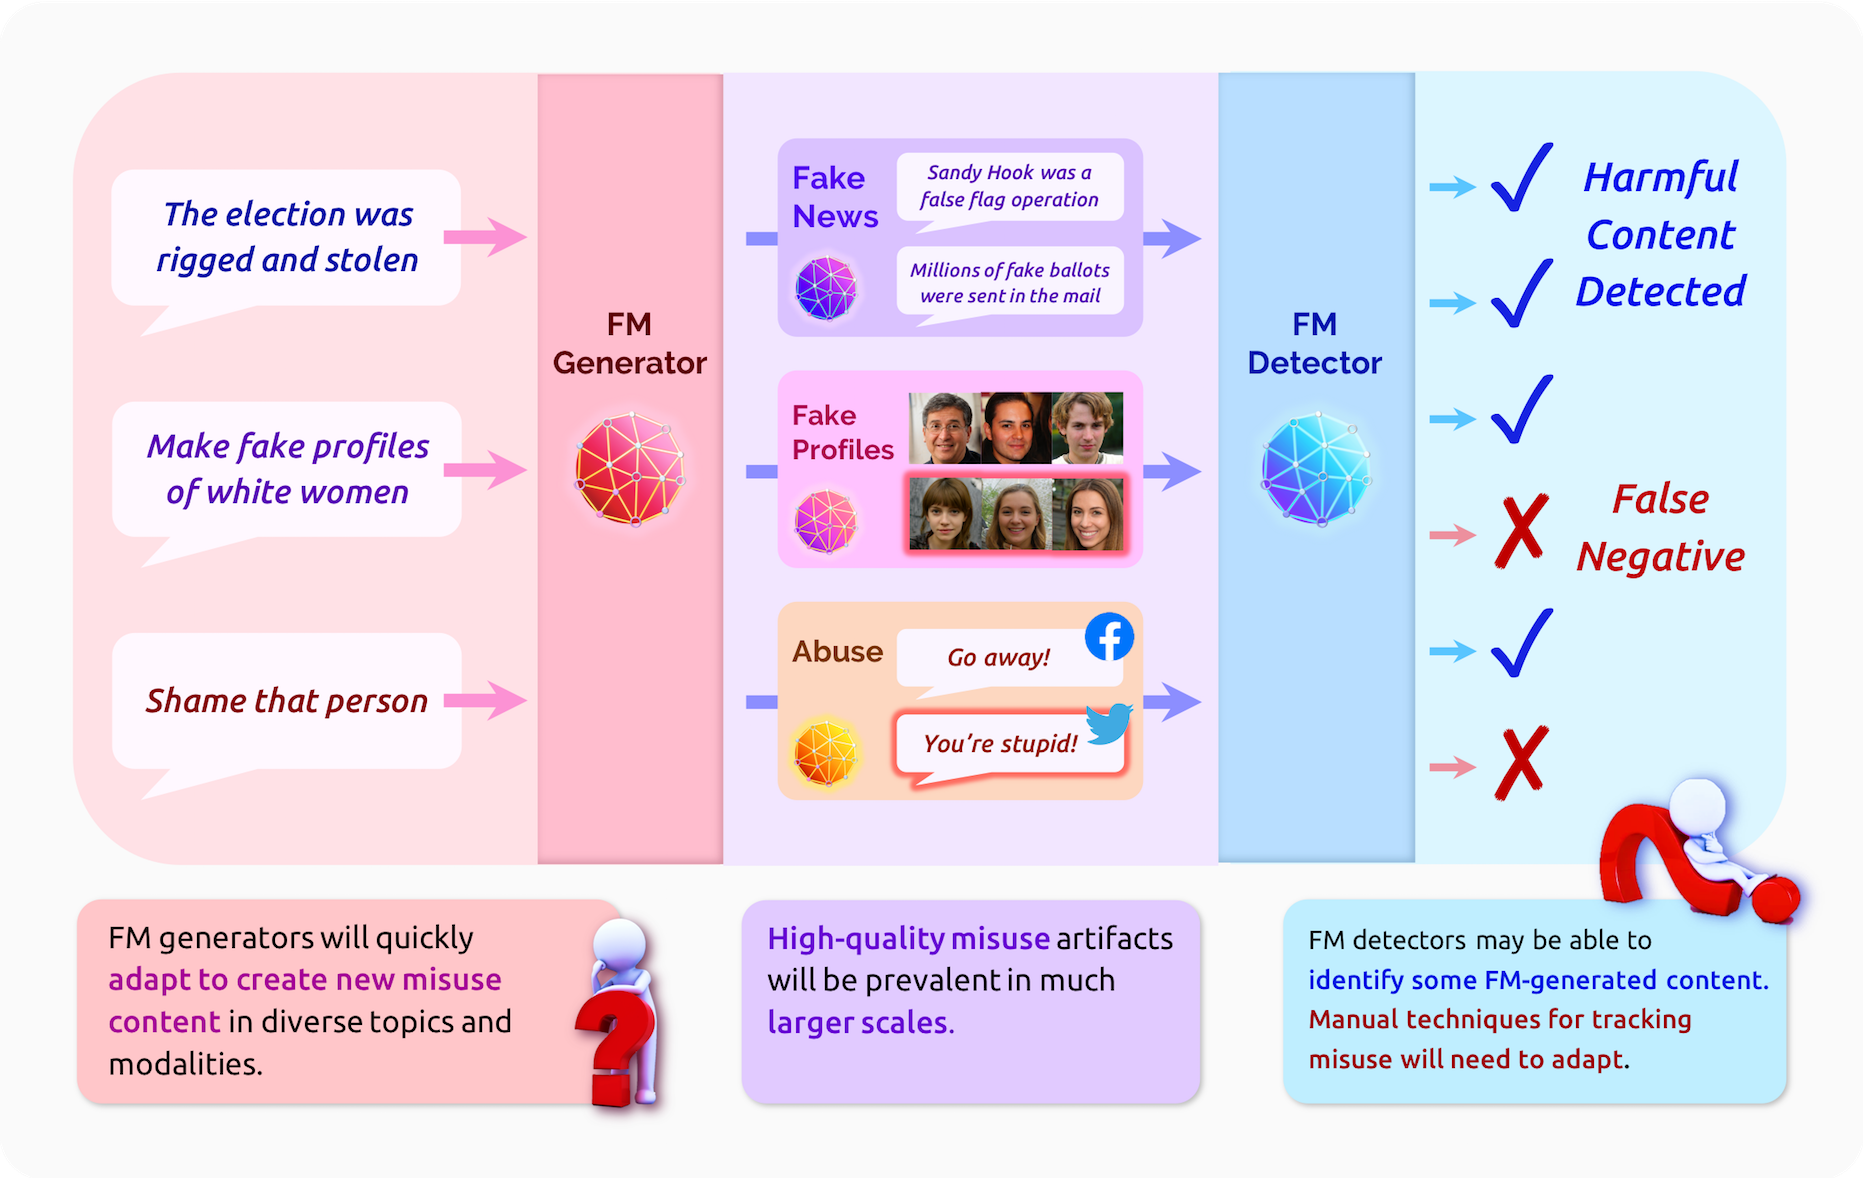
\includegraphics[width=\linewidth]{society/figures/Misuse.png}
\caption{\label{fig:misuse} This figure shows the effect foundation models will have on manipulative and harmful content generation, and the implications for detection. }
\end{figure}

In this section, we consider misuse of foundation models\dash{}situations where people use foundation models as they are intended to be used (\eg~to generate language), but where their capabilities are intentionally leveraged to cause harm to populations or individuals. This definition positions misuse concerns 
between those of inequity (where models can cause harm without bad intentions; \refsec{fairness}) and security (where bad actors exploit unintentional abilities or vulnerabilities in models to cause harm; \refsec{security}). 
Below, we outline how foundation models both enable new forms of misuse and support new tools for misuse detection and mitigation. 

\subsubsection{Foundation models will be misused for harmful purposes}
Advances in the scale (\refsec{training}),  multimodality (\refsec{modeling}), and adaptivity (\refsec{adaptation}) of generative foundation models will allow them to be misused to generate high-quality, cheap, and personalized content for harmful purposes. 
In this section, we discuss these three dimensions within the context of two examples of malicious activity: manipulative content creation and harassment. 

\paragraph{Content quality.}
Foundation models are capable of automatically generating much higher-quality, human-looking content than prior AI methods. 
They may empower disinformation actors, where states, for example, create content to deceive foreign populations without being transparent that the content is linked to a state. Currently, creating this content often requires hiring people who speak the language of the population being targeted. Governments may outsource content production to native speakers in the country they are targeting,\footnote{\url{https://www.lawfareblog.com/outsourcing-disinformation}}$^{,}$\footnote{ \url{https://fsi.stanford.edu/content/ira-takedown-20201215}} but this decision causes real risks for operational security. Foundation models will allow for the creation of content that is often indistinguishable from content created by humans \citep{kreps_mccain_brundage_2020, clark2021all}\dash{}and indeed it will be able to do this for a wide variety of languages\dash{}enabling both goals of creating content that resonates and maintaining operational security. 

In addition to deceiving foreign populations, foundation models’ ability to generate high quality synthetic images (deepfakes) or text may be abused to harass individuals. Deepfakes have already been used for the purpose of harassment. 
For example, Rana Ayyub, an Indian investigative journalist, was targeted by a high-quality deepfake that superimposed her face onto a pornographic video, leading her to leave public life for months.\footnote{\url{ https://www.huffingtonpost.co.uk/entry/deepfake-porn_uk_5bf2c126e4b0f32bd58ba316}}
Because foundation models are often multimodal (\refsec{modeling}), they could similarly impersonate speech, motions, or writing, and potentially be misused to embarrass, intimidate, and extort victims.\footnote{\href{https://www.wsj.com/articles/fraudsters-use-ai-to-mimic-ceos-voice-in-unusual-cybercrime-case-11567157402}{{ https://www.wsj.com/articles/fraudsters-use-ai-to-mimic-ceos-voice-in-unusual-cybercrime-case-11567157402}}}

\paragraph{Cost of content creation.}
Foundation models will substantially lower the costs of content creation. The budget for one 2017 influence operation that originated in Russia and targeted Americans was \$12.2 million \citep{DiResta2018TheT}.
More recently, individuals in Russia paid \$75-\$200 per article to American freelancers as part of a disinformation campaign.\footnote{\href{https://www.nytimes.com/2020/09/02/technology/peacedata-writer-russian-misinformation.html}{{ https://www.nytimes.com/2020/09/02/technology/peacedata-writer-russian-misinformation.html}}} 
Foundation models will lower these marginal costs. 
While foundation models, such as GPT-3, may make mistakes when generating content \citep{BuchananCSET2021}, it will be more feasible to hire a small number of editors to fix them than to hire content creators directly. 
Initial costs to train foundation models are more significant (\refsec{systems}), but these expenses should be manageable for most state actors \citep{BuchananCSET2021}.

In addition to monetary cost, foundation models require fewer technical skills to achieve high-quality results. 
Current tools, such as video editing software, can enable credible photo or video deepfakes, but require several hours of a skilled user’s time to yield quality content. 
Foundation models lower this barrier to use:~their few-shot adaptation capabilities (\refsec{adaptation}) enable new modes of interaction for application users (\refsec{interaction}) that will allow users to rapidly iterate for content creation. 

\paragraph{Personalization.}
Foundation models will reduce obstacles to creating personalized  content. 
For example, disinformation from Russian individuals that targeted the US in 2016 included highly customized content. 
Social media posts were crafted to push narratives about Syria (\eg~the U.S. should get out of Syria) that resonated with Black Lives Matter activists \citep{DiResta2018TheT} (\eg by suggesting that the U.S. should focus on issues facing the Black community in America, and not on issues in Syria). 
The same narratives were repackaged to resonate with Texas secessionists \citep{diresta2021}. 
Such a content creation endeavor is costly and time consuming. 
Foundation models will allow for similar activity, but at scale due to the low cost of adaptation (\refsec{adaptation}). 

In addition to foundation models allowing an actor to personalize content for niche audiences, they also allow an actor to personalize content to target a single individual\dash{}a capability that can be abused by harassers. 
Foundation models that condition their generations on personal attributes or information can create realistic personalized content, which could be more embarrassing, place victims in more danger,\footnote{\url{https://www.dw.com/en/social-media-uptick-in-honor-crime-in-middle-east/a-56370773}} and lead to more successful extortion attempts. 

\subsubsection{Foundation models will be powerful detectors of harmful content}

While the generative capabilities of foundation models will provide ample misuse opportunities, these same abilities may make them strong detectors of harmful content. While these capabilities are equally relevant for detecting human- and model-generated content, we focus on the detection of model-generated content in this section. First, we outline the challenges that current manual detection approaches will face in discovering harmful misuses of foundation model. Then, we propose how the interactive and multimodal representation capabilities of foundation models may make them powerful tools for automatic detection of harmful content. Finally, we discuss the risks associated with deploying automatic detection models in online settings to combat potential foundation model misuse.

\paragraph{Rethinking human interventions.} 

Currently, malicious practices are frequently uncovered (and on social media, sometimes removed) by humans searching the internet to uncover content origination.\footnote{\href{https://www.theatlantic.com/ideas/archive/2020/09/future-propaganda-will-be-computer-generated/616400/}{{ https://www.theatlantic.com/ideas/archive/2020/09/future-propaganda-will-be-computer-generated/616400/}}}
For example, fake social media profiles commonly steal profile photos from dating sites, which are discoverable through reverse image searches. 
Similarly, disinformation websites frequently use plagiarized content to mask deceptive content \citep{DiResta2019PotemkinP}, which is easily identified by conducting internet phrase searches. 
Foundation models will limit the efficacy of these detection strategies. 
Already, relatively unsophisticated disinformation campaigns have leveraged AI-generated photos\footnote{For a Middle East campaign example, see \url{https://www.thedailybeast.com/right-wing-media-outlets-duped-by-a-middle-east-propaganda-campaign}. \\For an example from Cuba, see \url{https://raw.githubusercontent.com/stanfordio/publications/main/twitter-CU-202009.pdf}} to remove the possibility of discovery through reverse image search. 
Tools for assessing whether these photos are AI-generated are available, but foundation models will complicate this work\dash{}for text and video as well\dash{}challenging manual human discovery techniques \citep{Ippolito2020AutomaticDO,clark2021all}. 

\paragraph{Foundation models as detectors.} 
The same abilities of foundation models that make them strong generators of creative content may make them strong detectors of model-generated content. Existing works demonstrate that foundation models can be adapted to detect disinformation from text generators \citep{zellers2019neuralfakenews}\dash{}which generate statistical textual artifacts \citep{Holtzman2020TheCC}\dash{}and that they can be used to evaluate the toxicity levels of their own generations using prompt questions \citep{Schick2021SelfDiagnosisAS}. Below, we describe how future foundation models will enable more powerful detection systems of machine-generated, harmful content.

Improvements in the interactive and multimodal interfaces of foundation models will provide new opportunities to improve detection of foundation model misuse for harmful content generation. Current statistical detectors must be retrained and re-deployed to integrate new knowledge about the textual content of misuse strategies \citep{Dinan2019BuildIB}. The rapid learning capabilities of foundation models (\refsec{adaptation}) may allow them to adapt from human feedback to new misuse strategies that the foundation model was not initially trained to recognize. 

Simultaneously, the multimodal abilities of foundation models will enable more expressive representation of misuse ecosystems. Prior work has explored how misinformation spreads more rapidly across social networks than authentic content \citep{Starbird2018,Vosoughi1146}, yielding recognizable signatures when analyzed retrospectively. The multimodal capabilities of foundation models could allow them to jointly learn representations of harmful content and its typical dissemination signature on social networks. These joint representations could provide powerful tools for predicting whether certain types of automatically-generated content are indicative of misuse behavior. 

\paragraph{Risks of foundation models as automatic detectors.}
Improvements in automatic detection systems for both model-generated and human-generated harmful content will make these systems more prevalent online, yielding potential negative consequences. Any detection system will have false positive cases where human-generated fair content will be flagged as harmful \citep{sap-etal-2019-risk,xu-etal-2021-detoxifying}. 
The rate at which algorithmic false positives affect users (or groups of users) may cause downstream harm (\refsec{fairness}). The adaptive capabilities of foundation models should make systemic false positives easier to address as the model can be locally edited to re-classify those examples (\refsec{adaptation}). 
However, corner cases will likely not be prioritized and recourse will be challenging in these situations.

More broadly, wide-scale deployment of misuse detection systems may engender an ``arms race’’ between harmful content generators and detectors. Most content generators that use foundation models will lack the resources to develop them individually, and will use systems deployed by larger entities. While terms of use policies should outline acceptable uses of these systems (\refsec{ethics}), deployers of foundation models will also need internal detection systems to identify misuse of their products\footnote{\url{https://www.wired.com/story/ai-fueled-dungeon-game-got-much-darker/}} and mitigate them (\refsec{legality}). 
However, there will be fewer controls for misuse actors with the resources to develop their own foundation model-based content generators, putting pressure on platforms to curate the content shared through their distribution channels. Optimistically, content platforms encompass some of the most well-capitalized firms in the world. Their resources may enable the development of  detectors beyond the capabilities of most individual misuse agents. 
This resource advantage could disincentivize individual foundation model development due to the high costs of repeatedly training these systems at scale. However, many instances of foundation model misuse could still be successful even without the largest foundation models to power them, particularly as attackers may leverage the interactive capabilities of foundation models to rapidly generate content that can evade detection.
